\begin{figure}[!htbp]
  \centering
  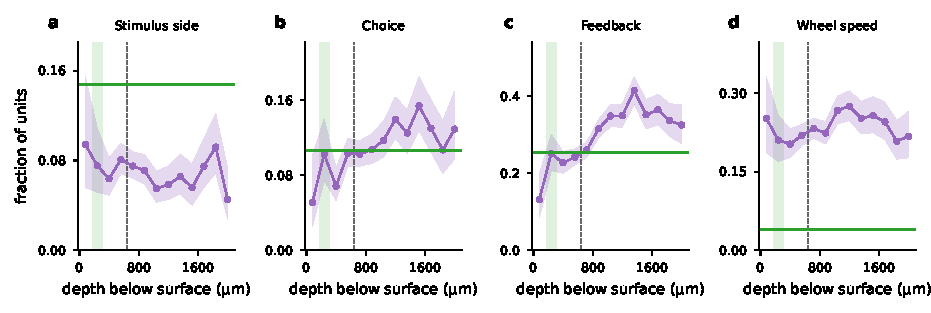
\includegraphics[width=\linewidth,height=0.8\textheight,keepaspectratio]{figures/depth.pdf}
  \caption{Depth sensitivity of the BWM comparison. Green line: mesoscope fraction over all neurons; green shading: mesoscope imaging depth (174--318\,$\mu$m, 5--95\,\% of the histology-registered sessions); dashed line: the 640\,$\mu$m cutoff of the depth-limited BWM set. Depth: Allen CCF top surface at the unit's ML-AP position minus its DV. \textbf{a} Fraction of BWM isocortex units tuned to stimulus side ($p<0.05$, same test as the maps) per 160\,$\mu$m depth band (purple; band: 95\,\% Wilson interval; bands with $\geq$30 units): 7.5\% of BWM units within 640\,$\mu$m, 6.7\% deeper, mesoscope 14.7\%. \textbf{b} Choice: 9.0\% of BWM units within 640\,$\mu$m, 11.4\% deeper, mesoscope 10.7\%. \textbf{c} Feedback: 23.3\% of BWM units within 640\,$\mu$m, 31.2\% deeper, mesoscope 25.4\%. \textbf{d} Fraction of units correlated with wheel speed ($r>0.1$ over the wheel bins of both the even and the odd trials): 21.5\% of BWM units within 640\,$\mu$m, 23.2\% deeper, mesoscope 4.0\%.}
  \label{fig:depth}
\end{figure}
